% 1977 年浙江卷第六题：△ABC 内一点 O，AO 延长交 BC 于 D（虚线），BO 延长交 AC 于 E、
% CO 延长交 AB 于 F（实线），OH 为 O 到 BC 的垂线段（虚线），K 为 A 的高线足，
% BC 上自左至右标 K、H、D（按源卷第 3 页布局）
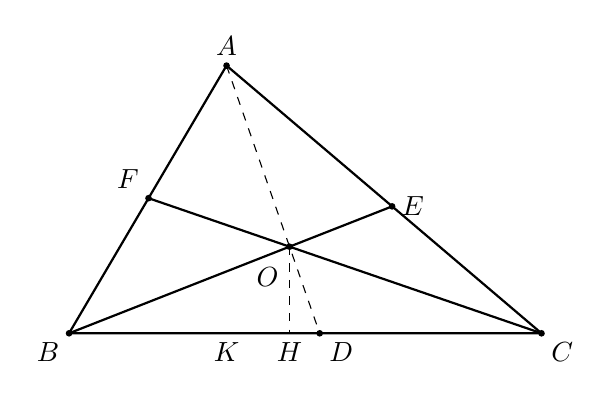
\begin{tikzpicture}[scale=1.0]
  \coordinate (A) at (2.0,3.4);
  \coordinate (B) at (0,0);
  \coordinate (C) at (6,0);
  \coordinate (O) at (2.8,1.1);
  \coordinate (D) at (3.183,0);
  \coordinate (E) at (4.103,1.612);
  \coordinate (F) at (1.009,1.716);
  \coordinate (K) at (2.0,0);
  \coordinate (H) at (2.8,0);
  \draw[thick] (A)--(B)--(C)--cycle;
  \draw[thick] (B)--(E);
  \draw[thick] (C)--(F);
  \draw[dashed] (A)--(D);
  \draw[dashed] (O)--(H);
  \fill (A) circle (1.2pt) node[above] {$A$};
  \fill (B) circle (1.2pt) node[below left] {$B$};
  \fill (C) circle (1.2pt) node[below right] {$C$};
  \fill (O) circle (1.2pt);
  \fill (D) circle (1.2pt) node[below right] {$D$};
  \fill (E) circle (1.2pt) node[right] {$E$};
  \fill (F) circle (1.2pt) node[above left] {$F$};
  \node[below] at (K) {$K$};
  \node[below] at (H) {$H$};
  \node at (2.52,0.72) {$O$};
\end{tikzpicture}
